
%\section{Computation and Communication Overheads in ReLU Computation} \label{sec:ReluOverhead}
%
%The computation and communication (between server and client in two party computation settings) overheads of individual  ReLU and convolution (Conv) operation is shown in Table \ref{tab:ReluOverheads}. These (amortized) values are calculated according to the Table 1 and Table 3 in  DELPHI \cite{mishra2020delphi}. Clearly, ReLU operation has orders of magnitude higher computation and communication overheads (especially in online phase) compared to the convolution operations. Therefore, removing ReLUs from networks (with minimal impact on accuracy)  is a paramount importance for the private inference. 
%\input{42AppendixTable_ReluOverheadComp}


\section{Channel Scaling Vs. Feature map Scaling} \label{secAppendix:ChannelVsFmapScaling}


For extremely lower ReLU budgets, we use a combination of channel scaling and fmaps' resolution scaling. Since reducing  fmaps' resolution (each spatial dimensions of fmaps) by 2$\times$ ($\rho$=0.5) decreases the ReLU count by 4$\times$, we first use channel scaling ($\alpha$ = 0.5) for reducing the ReLU count by 2$\times$. Further, for 4$\times$ reduction in ReLU count, we prefer to use fmaps' resolution scaling ($\rho$=0.5) over channel scaling ($\alpha$=0.25) since the former results in more accurate networks, as illustrated in Table \ref{tab:AlphaVsRhoComp}. Unlike fmap resolution scaling, channel scaling reduces the parameter count along with the ReLU count, which may reduce the expressive power of a network. Hence, the network is more accurate with fmaps' resolution scaling.  
  
\begin{table} [htbp]
\caption{Performance comparison for ReLU optimization using channel scaling ($\alpha<$1) and fmap-resolution scaling ($\rho<$1). Baseline models have $\alpha$=1 and $\rho$=1. At iso-ReLU, accuracy (w/ KD) of the the fmap-resolution scaled models is higher than the channel scaled models.}
\label{tab:AlphaVsRhoComp}
\centering 
\resizebox{0.49\textwidth}{!}{
\begin{tabular}{ccccc} 
 \toprule
\multirow{2}{*}{Network} & \multirow{2}{*}{\#Conv} & \multirow{2}{*}{\#ReLUs} & \multicolumn{2}{c}{CIFAR-100} \\
\cmidrule(lr{0.5em}){4-5}  
& & & {W/o KD (\%)} & {W/ KD (\%)} \\
 \toprule
ResNet18 (baseline) & 17 & 557K & 74.46 & 76.94 \\
ResNet18; $\alpha$=0.25, $\rho$=1  & 17 & 139K & 68.17 & 70.19 \\
ResNet18; $\alpha$=1, $\rho$=0.5 & 17 & 139K & 68.47 & 72.72 \\ \midrule
ResNet10 (baseline)& 9 & 311K & 74.10 & 76.69 \\
ResNet10; $\alpha$=0.25, $\rho$=1 & 9 & 78K & 66.69 & 66.88 \\ 
ResNet10; $\alpha$=1, $\rho$=0.5 & 9 & 78K & 66.67 & 71.86 \\ \midrule
ResNet6 (baseline) & 5 & 188K & 68.86 & 69.58 \\
ResNet6; $\alpha$=0.25, $\rho$=1 & 5 & 47K & 57.64 & 56.9 \\
ResNet6; $\alpha$=1, $\rho$=0.5 & 5 & 47K & 64.74 & 68.09 \\ 
\bottomrule
\end{tabular}} 
\end{table}





\section{VGGNet DeepReDuce Pareto Points} \label{SecAppendix:ParetoPointsVGG16}

We do not remove ReLUs from fully connected (FC) layers as FC account only 8.192K ReLUs and training networks without FC ReLUs is challenging. The results are shown in Table \ref{tab:ReluCriticalityVGG16}. Unlike ResNets and MobileNets, ReLUs in $S_5$ are least critical and that of the $S_1$ is moderate. 

\begin{table} [htbp]
\caption{Stage-wise ReLUs' criticality  in VGG16 evaluated on CIFAR-10. $S_5$ is least critical while $S_2$ and $S_3$ are most critical.}
\label{tab:ReluCriticalityVGG16}
\centering 
\resizebox{0.49\textwidth}{!}{
\begin{tabular}{ccccc} \toprule
Net & \#ReLUs & W/o KD (\%) & W/ KD (\%) & $C_k$ \\ \toprule
%Baseline & 284.7 & 93.71 & & \\ \midrule
$S_1$ + FC-ReLUs & 139.3K & 82.0 & 81.4 & 10.90 \\
$S_2$ + FC-ReLUs & 73.7K & 86.1 & 85.3 & 14.31 \\
$S_3$ + FC-ReLUs & 57.3K & 86.4 & 85.1 & 14.40 \\
$S_4$ + FC-ReLUs & 32.8K & 77.1 & 77.7 & 9.17 \\
$S_5$ + FC-ReLUs & 14.3K & 63.9 & 66.0 & 0.00 \\ 
\bottomrule
\end{tabular} }
\end{table}



The ReLU optimizations step for the Pareto points in Figure \ref{fig:ParetoFrontierVGG16} are listed in Table \ref{tab:ParetoPointsVGG16}.  Models are the ReLU-optimized versions (Thinned and Reshaped) of two Culled networks: (1) stages $S_4$ and $S_5$ are Culled and (2) stages $S_1$, $S_4$ and $S_5$ are Culled. 

\begin{table} [htbp]
\caption{Optimization steps for MobileNetV1 DeepReDuce models shown in Figure  \ref{fig:ParetoFrontierVGG16}}
\label{tab:ParetoPointsVGG16}
\centering 
\resizebox{0.49\textwidth}{!}{
\begin{tabular}{lcc} \toprule
Optimization Steps & \#ReLUs & Acc.(\%) \\ \toprule
$S_1$ + $S_2$ + $S_3$ + FC & 253.95K & 93.92 \\
$S_2$ + $S_3$ + FC & 122.88K & 92.52 \\
$S_2^{RT}$ + $S_3^{RT}$ + FC & 73.73K & 90.23 \\
$S_1^{RT}$ + $S_2^{RT}$ + $S_3^{RT}$ + FC, $\alpha$=0.5 & 69.63K & 89.97 \\
$S_2^{RT}$ + $S_3^{RT}$ + FC, $\alpha$=0.5 & 36.86K & 88.92 \\   \bottomrule
\end{tabular} }
\end{table}





\section{ReLUs' Criticality and Pareto Points for MobileNets} \label{SecAppendix:ParetoPointsMV1}


We evaluate the ReLUs' criticality in MobileNetV1 \cite{howard2017mobilenets} and MobileNetV2 \cite{sandler2018mobilenetv2}) on the CIFAR-100. The results are shown in Table \ref{tab:CriticalityInMobileNets}.  We observed the similar trend as ResNet18 and ResNet34 on CIFAR-100/TinyImageNet (shown in Tables \ref{tab:ReluHeteroR18} and \ref{tab:ResNetBlockDropout}), accuracy differs significantly across stages and $S_1$ ($S_4$) ReLUs are least (most) critical.
\begin{table} [htbp] \centering
\caption{Stage-wise criticality of ReLUs in MobileNetV1 and MobileNetV2 evaluated on CIFAR-100. FR is baseline with Full-ReLU ($S_1$+$S_2$+$S_3$+$S_4$+$S_5$). ReLUs in $S_1$ ($S_4$) are least (most) critical.}
\label{tab:CriticalityInMobileNets} 
\resizebox{.5\textwidth}{!}{
\begin{tabular}{ccccccccc} \toprule
\multirow{2}{*}{ Net } & \multicolumn{4}{c}{ MobileNetV1 } & \multicolumn{4}{c}{ MobileNetV2 } \\ 
\cmidrule(lr{0.5em}){2-5}  
\cmidrule(lr{0.5em}){6-9} 
& \#ReLUs & W/o KD(\%) & W/ KD(\%) & $C_k$ &\#ReLUs & W/o KD(\%) & W/ KD(\%) & $C_k$ \\ \toprule
FR & 411.6K & 67.58 & - &    -   &425.6K & 68.46 & -     &  - \\ 
$S_1$ & 131.1K & 33.06 & 34.16 & 0.00 & 196.6K & 37.82 & 34.25 & 0.00 \\
$S_2$ & 114.7K & 49.64 & 50.65 & 11.83 & 110.6K & 49.83 & 46.93 & 9.12 \\
$S_3$ & 57.3K & 55.56 & 54.20 & 15.09 & 58.4K & 54.74 & 53.06 & 14.15 \\
$S_4$ & 94.2K & 57.37 & 61.10 & 19.60 & 27.6K & 57.08 & 57.28 & 18.26 \\
$S_5$ & 14.3K & 42.32 & 45.45 & 9.37 & 32.4K & 48.42 & 50.49 & 12.73 \\  \bottomrule
\end{tabular} }
\end{table}


The Pareto points of DeepReDuce models for MobileNetV1 (CIFAR-100) are shown in Figure \ref{fig:ParetoFrontierMV1}. The optimization steps for all DeepReDuce models are list in the Table \ref{tab:ParetoPointsMV1}. 


First, in step 1 of DeepReDuce (Figure \ref{fig:BlockDiagramDeepReDuce}), we Culled the least critical stage $S_1$. In step 2 of ReLU Thinning, we had two ways to remove the ReLUs from alternate layers, either from $3\times3$ depthwise convolution layer or $1\times1$ pointwise convolution layer. When downsampling is performed in $3\times3$ depthwise convolution layer, the ReLU count of both the layers are not equal. More precisely, \#ReLUs in the $1\times1$ pointwise convolution is twice as that in the preceding $3\times3$ depthwise conv. 


We empirically found that removing ReLUs from $3\times3$ depthwise conv layer yields more accurate iso-ReLU models. We suspect this is because $3\times 3$ depthwise convolutions perform filtering (feature learning) and $1\times1$ pointwise convolutions perform feature aggregation \cite{howard2017mobilenets}, the ReLUs in the former layer is more critical for accuracy. 


\begin{table} [htbp]
\caption{Optimization steps for MobileNetV1 DeepReDuce models shown in Figure  \ref{fig:ParetoFrontierMV1}}
\label{tab:ParetoPointsMV1}
\centering 
\resizebox{0.49\textwidth}{!}{
\begin{tabular}{lcc} \toprule
Optimization Steps & \#ReLUs & Acc.(\%) \\ \toprule
$S_2$ + $S_3$ + $S_4$ + $S_5$ & 280.60K & 70.83 \\
$S_2^{RT}$ + $S_3^{RT}$ + $S_4^{RT}$ + $S_5^{RT}$ & 108.54K & 70.77 \\
$S_2^{RT}$ + $S_3^{RT}$ + $S_4^{RT}$ + $S_5^{RT}$, $\alpha$=0.5 & 54.27K & 67.46 \\
$S_2^{RT}$ + $S_3^{RT}$ + $S_4^{RT}$ + $S_5^{RT}$, $\rho$=0.5 & 27.14K & 62.96 \\
$S_2^{RT}$ + $S_3^{RT}$ + $S_4^{RT}$ + $S_5^{RT}$, $\alpha$=0.5, $\rho$=0.5 & 13.57K & 58.25 \\  \bottomrule
\end{tabular} }
\end{table}




\section{ReLU Criticality in ResNet56} \label{SecAppendix:ReluCriticalityInR56}

We examine the stage-wise criticality of ReLUs in ResNet56 and results are shown in Table \ref{tab:ReluCriticalityR56}. 


\begin{table} [htbp]
\caption{Stage-wise criticality of ReLUs in ResNet56 evaluated on CIFAR-100. $S3$ is most critical and $S1$ is least critical.}
\label{tab:ReluCriticalityR56}
\centering 
%\resizebox{0.49\textwidth}{!}{
\begin{tabular}{ccccc} \toprule
Stages & \#ReLUs & W/o KD (\%) & W/ KD (\%) & $C_k$ \\ \toprule
S1 & 311.3K & 57.92 & 59.45 & 0.0 \\
S2 & 147.5K & 65.62 & 67.97 & 6.0 \\
S3 & 73.73K & 65.36 & 69.22 & 7.2 \\ \bottomrule
\end{tabular} 
\end{table}




\section{Layer-wise Distribution of ReLUs} \label{secAppendix:LayerWiseOpsInDNNs}

We show the layer-wise distribution of FLOPs, parameters, and ReLU count in the standard networks such as ResNet34 \cite{he2016deep}, VGG16 \cite{simonyan2014very}, MobileNetV1 \cite{howard2017mobilenets}, and MobileNetV2 \cite{sandler2018mobilenetv2} in Figure \ref{fig:LayerWiseReluInOtherDNNs}. Consistent with ResNet18 (Figure \ref{fig:LayerWiseReluInDNNs}), the FLOPs are evenly distributed, more parameters are used in deeper layers, and ReLUs are mostly in initial layers of the networks. Thus, the ReLU reduction in initial layers has a significantly greater impact on the overall ReLU count of these networks. Moreover, the stark difference between the ReLU distribution and FLOPs/parameter distribution indicates that ReLU optimization cannot be ensured through the popular FLOPs/parameters pruning techniques. 

%\begin{figure*}[htbp] 
%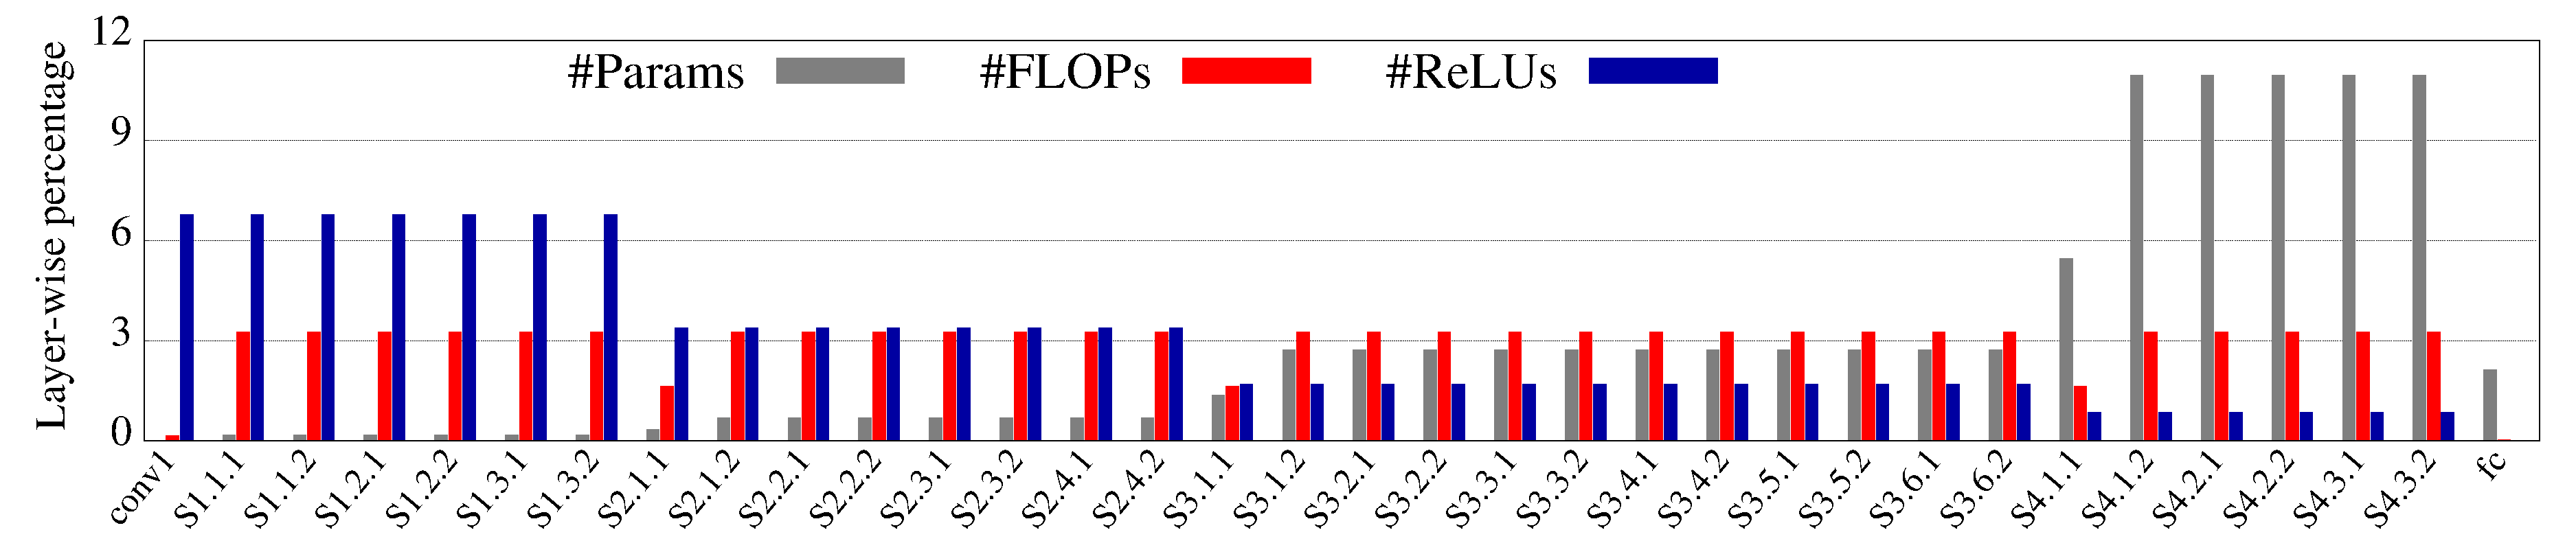
\includegraphics[scale=0.27]{Figures/LayerWiseOps_R34} 
%%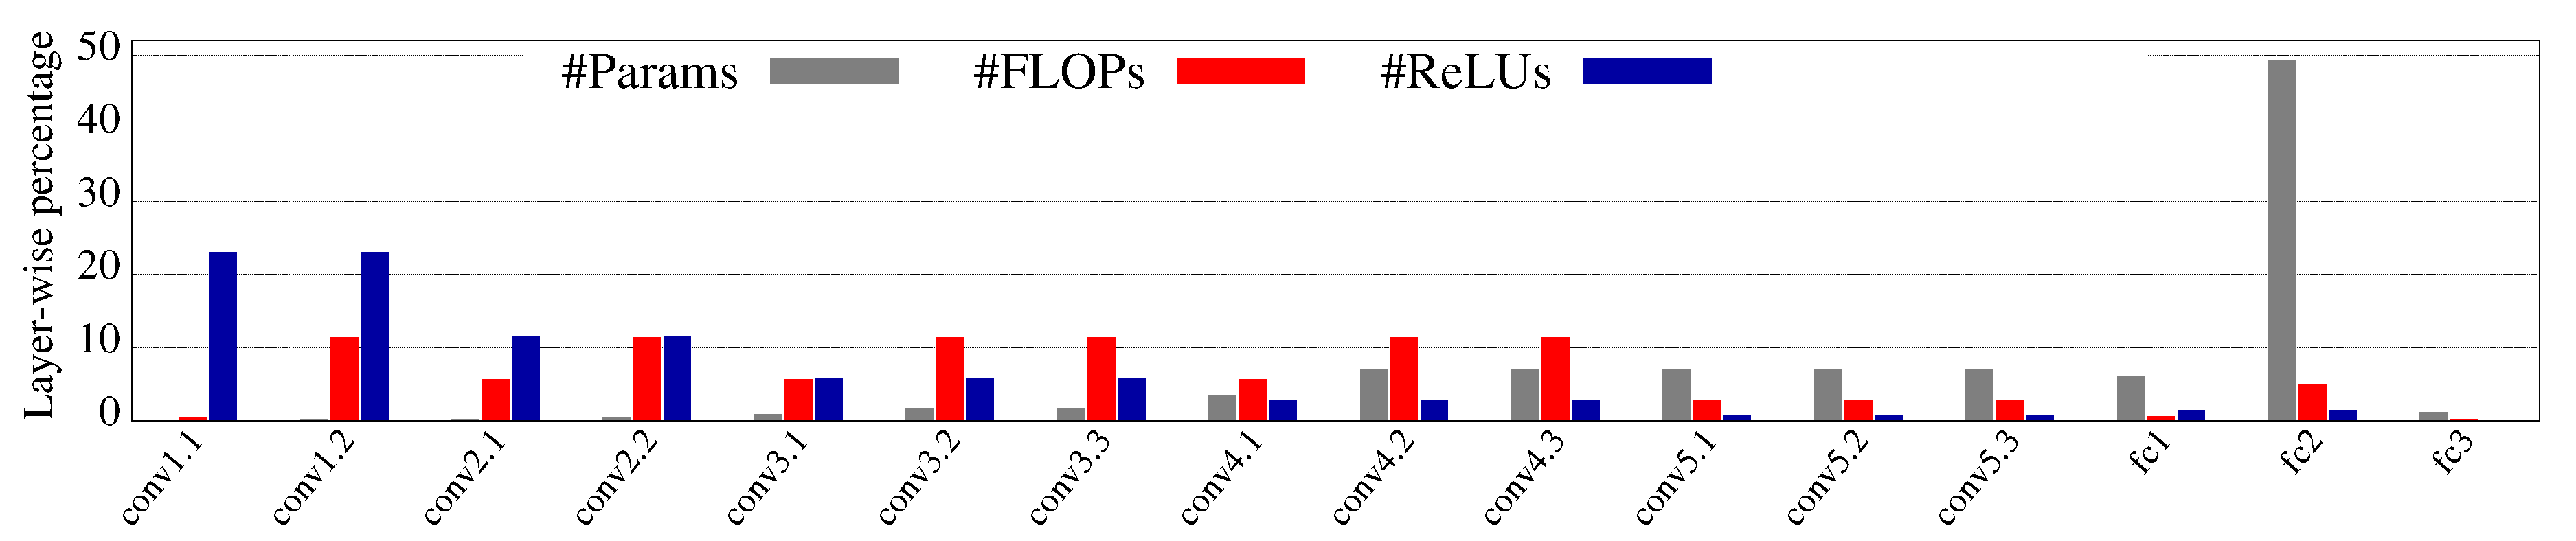
\includegraphics[scale=0.27]{Figures/LayerWiseOps_Vgg16}   \\ 
%%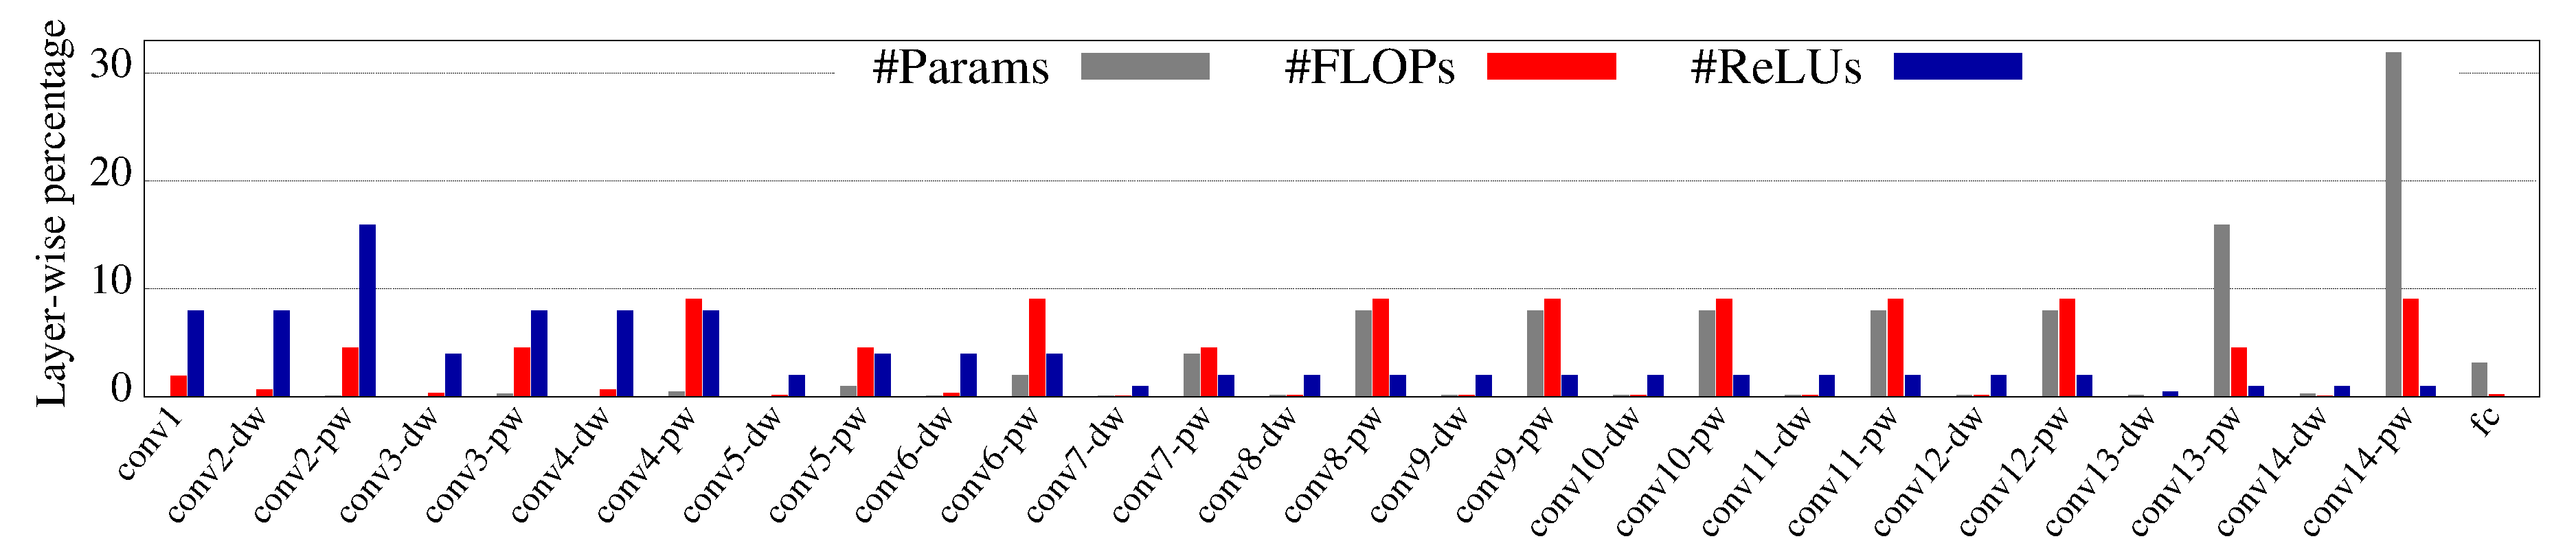
\includegraphics[scale=0.16]{Figures/LayerWiseOps_MV1} 
%%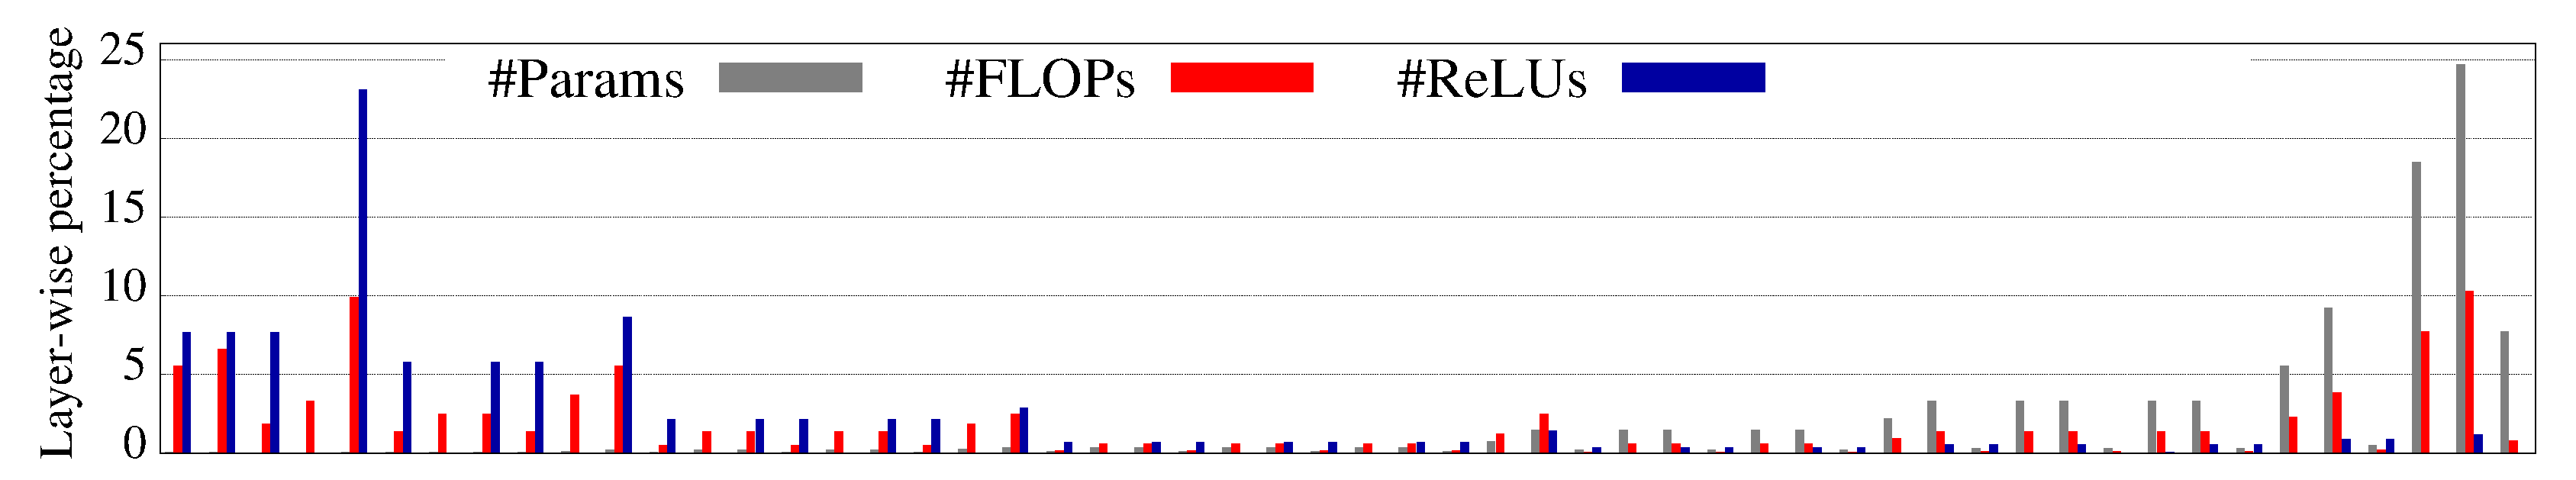
\includegraphics[scale=0.18]{Figures/LayerWiseOps_MV2}
%\caption{
%Layer-wise distribution of parameter, FLOPs, and ReLUs for ResNet34 (top-left), and VGG16 (top-right); and MobileNetV1 (bottom left) and MobileNetV2 (bottom right). FLOPs are evenly distributed, parameters (ReLUs) are increases (decreases) from initial to deeper layers. }
%\label{fig:LayerWiseReluInOtherDNNs}
%\end{figure*}

\begin{figure*}
\begin{subfigure}{1.0\textwidth}
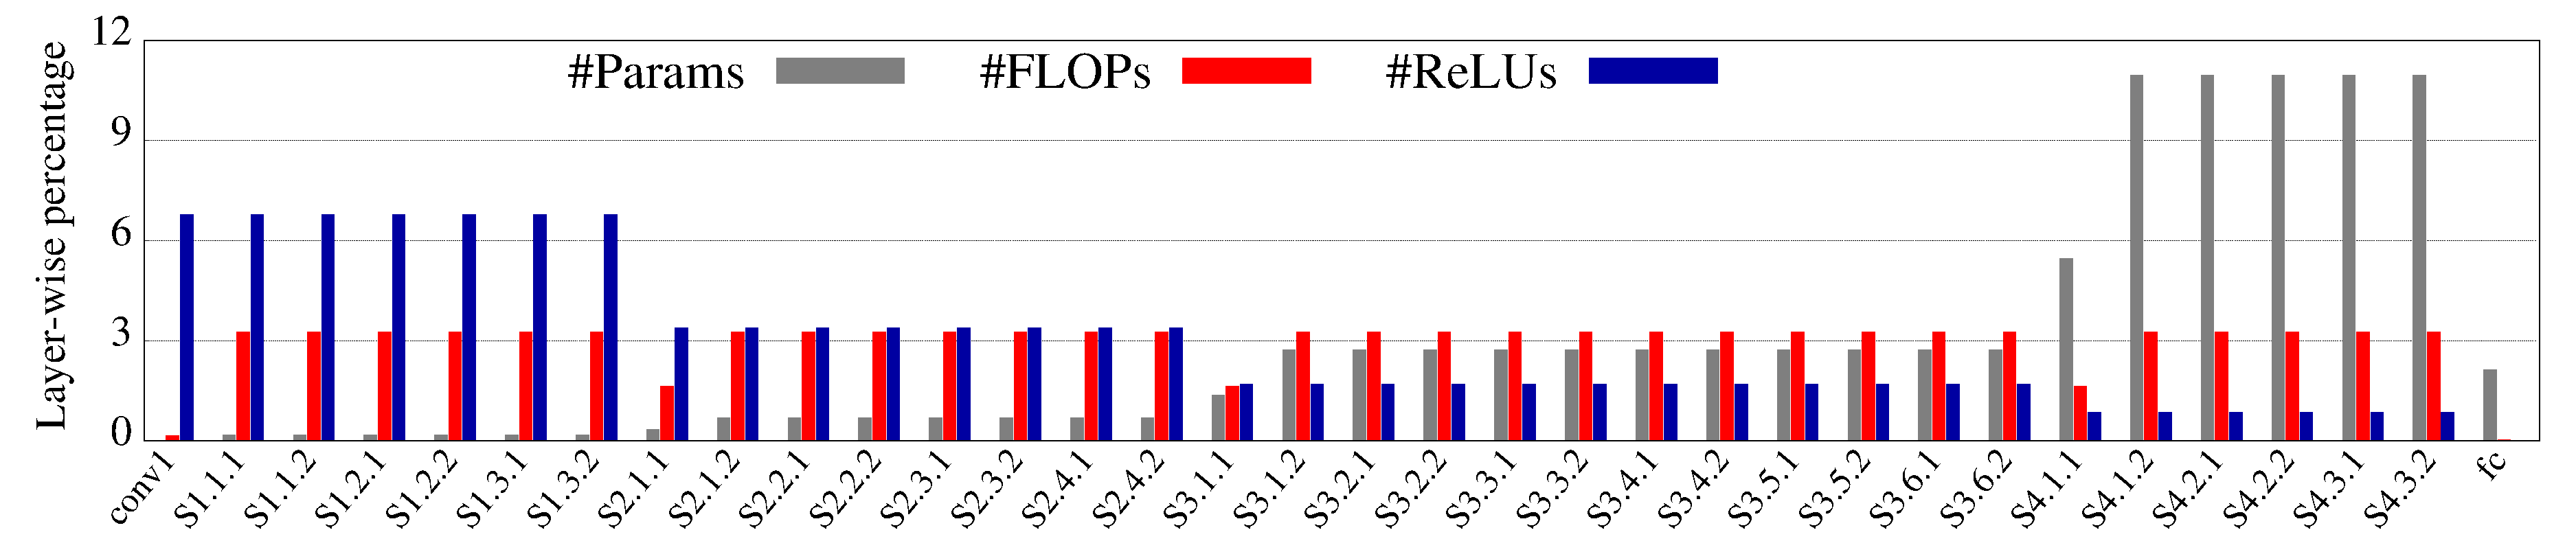
\includegraphics[scale=0.27]{Figures/LayerWiseOps_R34}
\caption{Layer-wise distribution of parameter, FLOPs, and ReLUs in ResNet34 \cite{he2016deep}.} \label{fig:LayerWiseReluInOtherDNNs_a}
\end{subfigure} \\
\begin{subfigure}{1.0\textwidth}
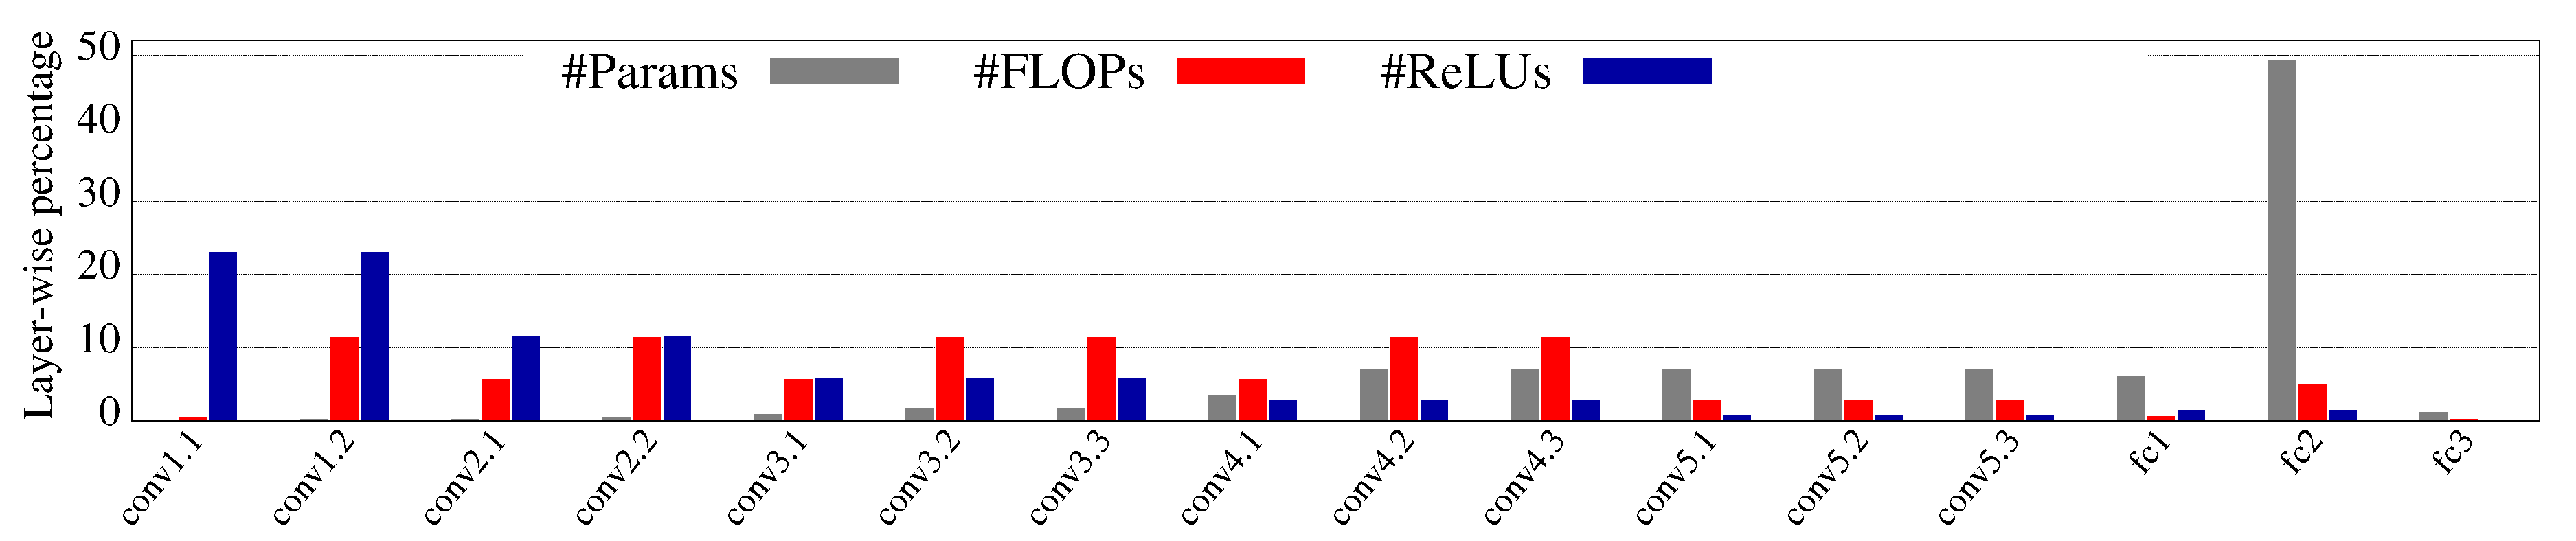
\includegraphics[scale=0.27]{Figures/LayerWiseOps_Vgg16}
\caption{Layer-wise distribution of parameter, FLOPs, and ReLUs in VGG16 \cite{simonyan2014very}.} \label{fig:LayerWiseReluInOtherDNNs_b}
\end{subfigure} \\
\begin{subfigure}{1.0\textwidth}
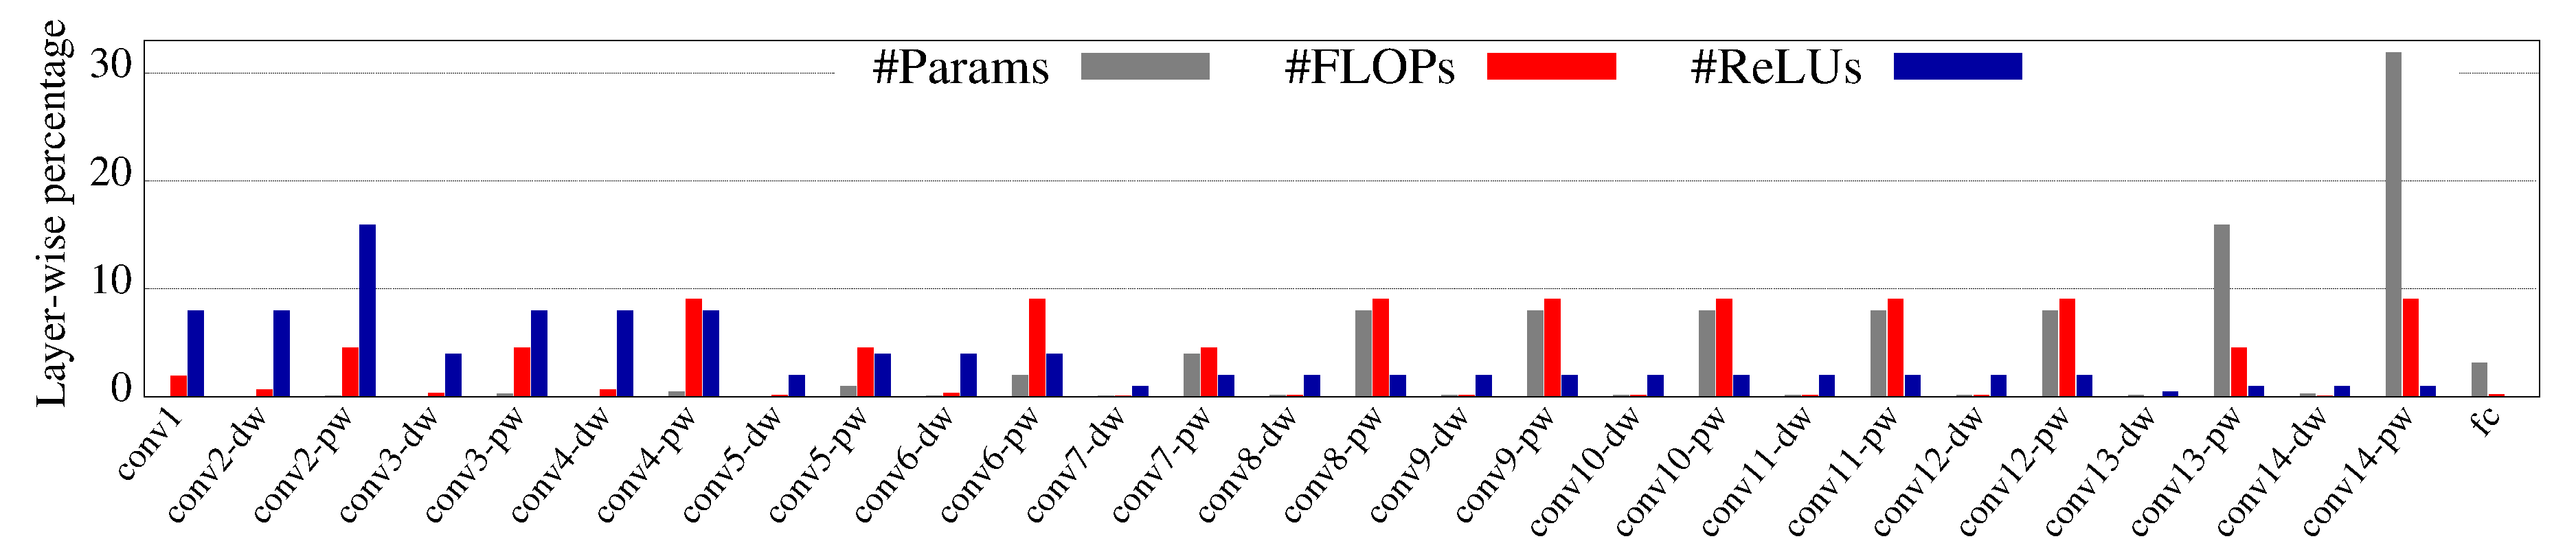
\includegraphics[scale=0.27]{Figures/LayerWiseOps_MV1}
\caption{Layer-wise distribution of parameter, FLOPs, and ReLUs in MobileNetV1 \cite{howard2017mobilenets}.} \label{fig:LayerWiseReluInOtherDNNs_c}
\end{subfigure} \\
\caption{Layer-wise percentage of parameter, FLOPs, and ReLUs in various DNNs. FLOPs are evenly distributed, parameters (ReLUs) are increases (decreases) from initial to deeper layers.} 
\label{fig:LayerWiseReluInOtherDNNs}
\end{figure*}

